
\subsection{Data Subsection}
\blindtext

\subsection*{Examples how to cite}

Here I give some examples how to cite:
\cite{moore_campylobacter_2005}
\parencite{moore_campylobacter_2005} 
\textcite{moore_campylobacter_2005}
\citeauthor{moore_campylobacter_2005}
\citetitle{moore_campylobacter_2005}

\subsection*{How to add an image}

\begin{figure*}[!ht]
	\centering
	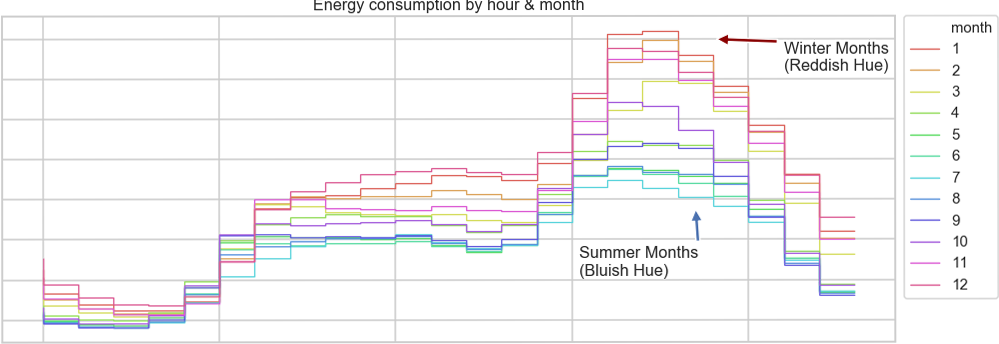
\includegraphics[width=\textwidth]{images/testimage1}
	\caption{This is an image}
	\label{fig:testimage1}
\end{figure*}

\begin{figure*}[!ht]
	\centering
	\subfloat[A floating image]{{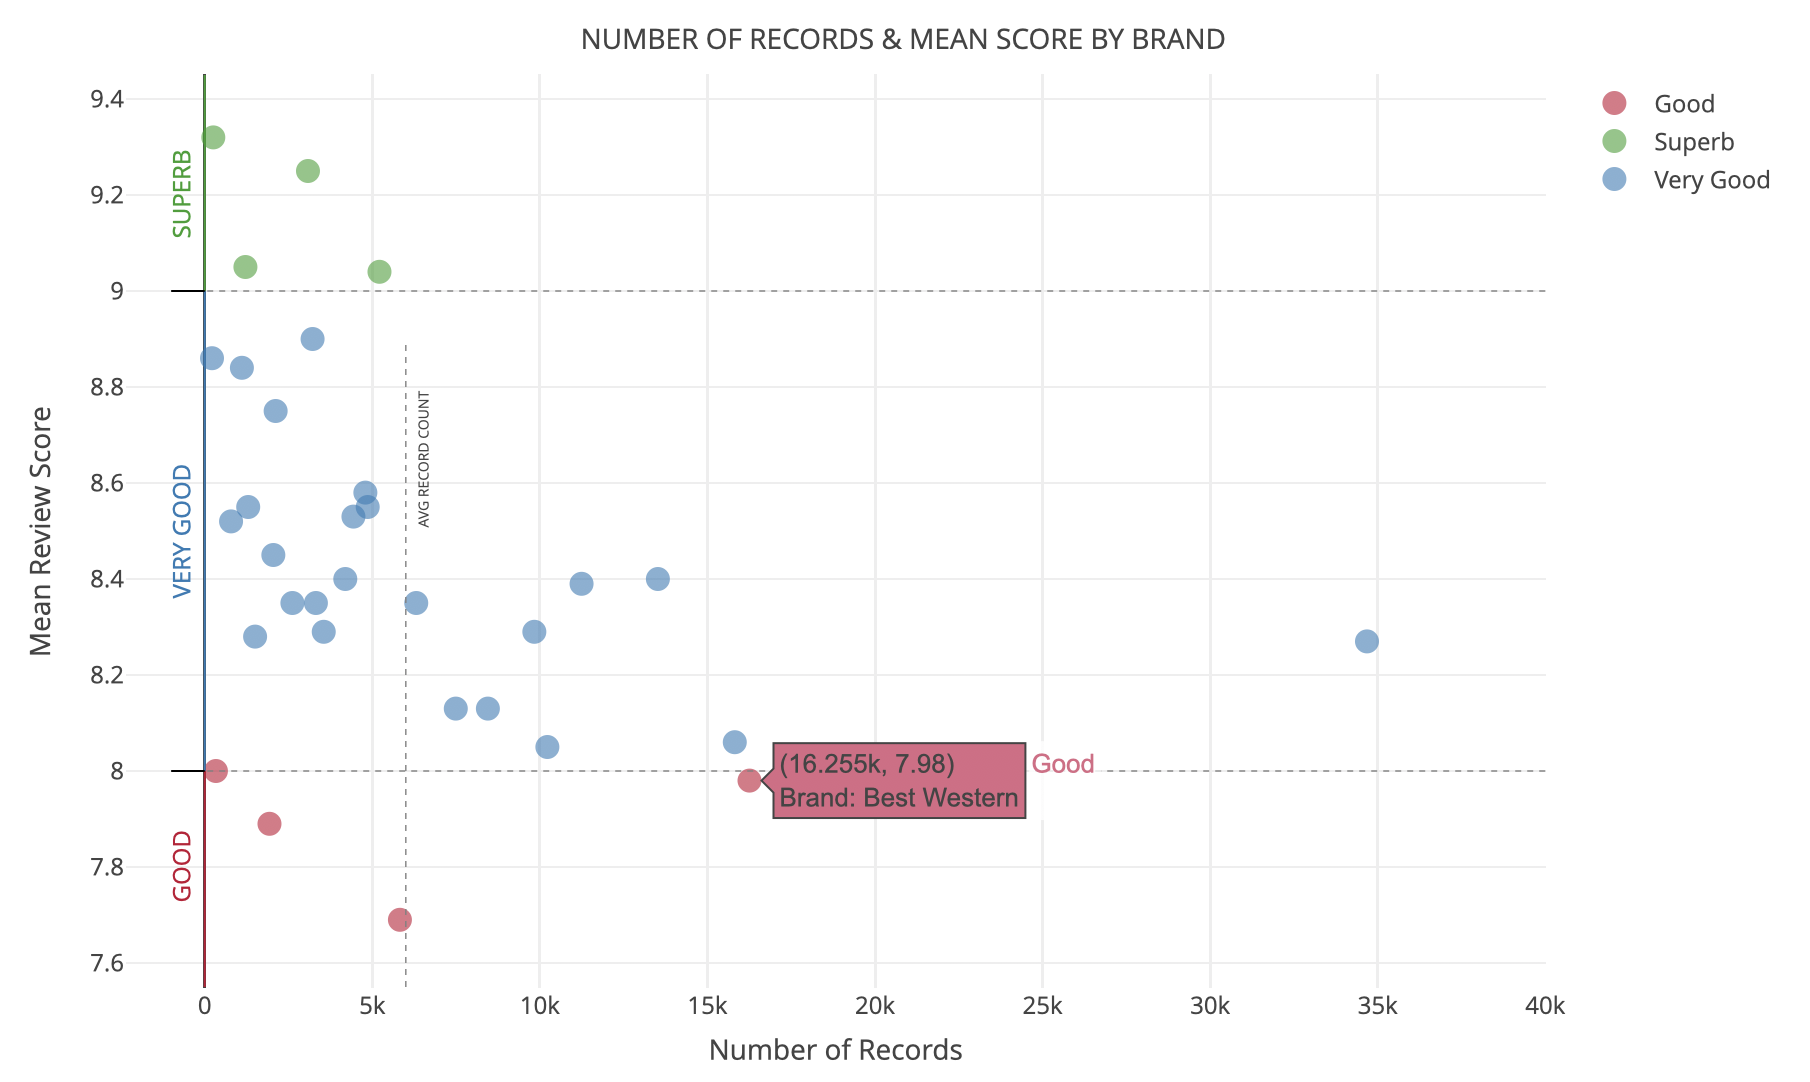
\includegraphics[width=0.45\textwidth]{images/testimage3_1} }}%
	%	\qquad
	\subfloat[Another image ]{{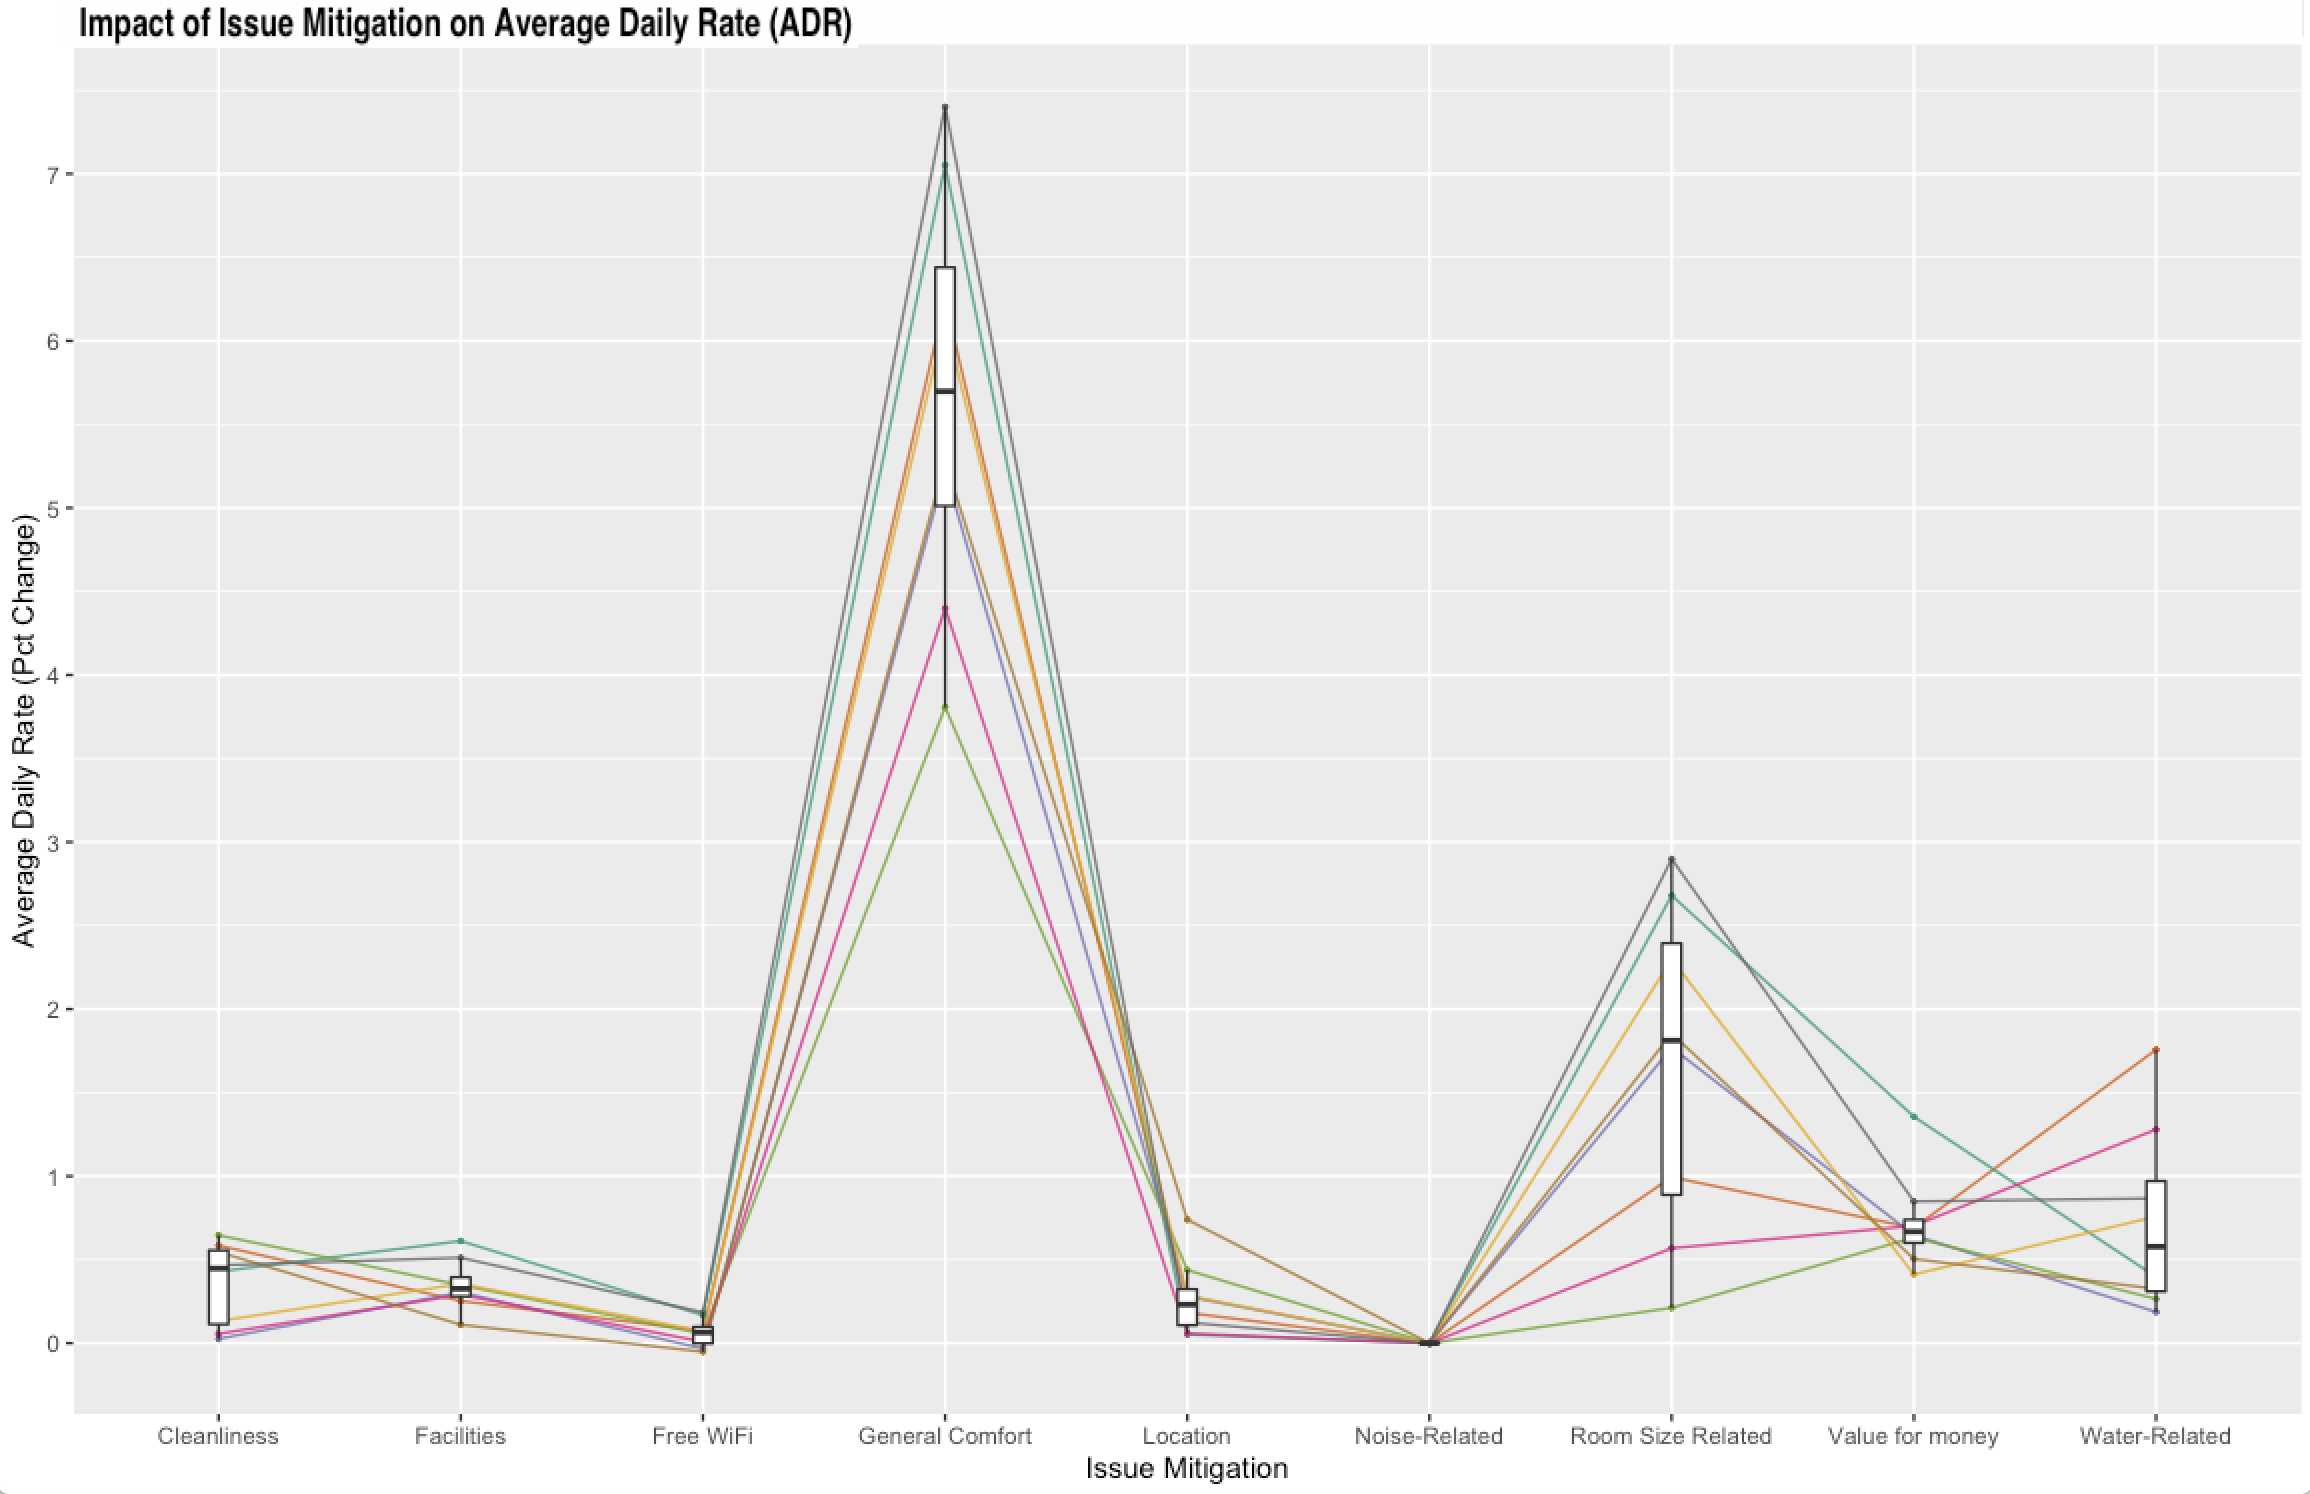
\includegraphics[width=0.45\textwidth]{images/testimage3_2}}}%
	\caption{Floating Images}%
	\label{fig:floatimage}%
\end{figure*}
\iffalse
1.	Explain basics of SD
    a.	Basics of SD
    b.	Examples from literature to clarify and justify modelling choices given problem in the field
2.	Conceptualisation
    a.	Depict aggregate model structure
    b.	Describe dynamic hypothesis
3.	Explain model (also refer to Appendix A)
    a.	Describe sub-models
    b.	Explain most important assumptions
4.	Validation
    a.	Use various tests to argue why model is fit for purpose
5.	Experimental setup
    a.	Introduce main uncertainties (potentially with table)
    b.	Explain scenario and policy logic
    c.	Number of runs, numerical integration method & time step, versions, etc.: all justified
\fi


\subsection*{How to equation}

Split Line in Equations
\begin{equation}
\begin{split}
\label{eqn:natsec}
ln(GVA_{Sector}) = \beta_1ln(SumOfLights)_{t}+\beta_2ln(SumElectricity)_t +\\ \beta_3ln(SumOfLightsSq)_{t} + \beta_4ln(Population)_{t} +
\alpha_i + u_{it}
\end{split}
\end{equation}

Aligned Equations
$$
\begin{aligned}
y_t &= 10.3009 -0.0042x_L - 0.0045x_B - 0.0032x_c -0.0046x_{d1} + \ldots + 0.0176x_{d6} + \eta_t \\
\eta_t &= 0.9146\eta_{t-1} + \epsilon_t -0.5015\epsilon_{t-1}\\
\epsilon_t &= \sim \text{NID}(0,0.003443)
\end{aligned}
$$

{\Huge \textcolor{pink}{FEEL FREE TO ASK ME QUESTIONS - Z}}